\documentclass[italian]{RMcv}
%
\hypersetup{%
    hidelinks,%
    colorlinks=false,%
    pdfauthor={Riccardo Milani},%
    pdftitle={CV Milani},%
    pdfdisplaydoctitle=true,%
    %pdfsubject={CV},
    pdfkeywords=CV,%
    %pdfpagemode=FullScreen,%
    %pdfmenubar=false,%
    %pdftoolbar=false,%
    pdflang=it-IT,%
    pdfcreator=LaTeX,%
}

%\renewcommand\intracvevent{4pt} % Spacing between a cvevent and the previous object. Default: 6pt
%\renewcommand\intercvevent{4pt} % Spacing between first line and bullet point of a cvevent. Default: 6pt

\title{CV - Ita}

\newif\ifcvtitle
\newif\ifcvsubtitle
\cvtitlefalse
\cvsubtitlefalse

%============================================================================%
%
%
%
%  DOCUMENT CONTENT
%
%
%
%============================================================================%
\begin{document}

%---------------------------------------------------------------------------------------
%  TITLE HEADLINE
%----------------------------------------------------------------------------------------
\vspace{-20.55pt}

\cvhead{CV}

\vspace{2px}
\center{%
 \ifcvtitle{Ingegnere Matematico $\cdot$} \fi%
 Italiano, Francese $\cdot$ %\faFlag~
 15/01/1991 $\cdot$ %
 Lecco $\cdot$ %
 \href{mailto:ricc.milani@gmail.com}{\textcolor{sectcol}{\textbf{ricc.milani@gmail.com}}} $\cdot$ %\faEnvelope
 {+33 7 83 93 34 47} $\cdot$ %\faPhone or \faMobilePhone\footnotesize
 \textcolor{sectcol}{\faLinkedinSquare\href{https://www.linkedin.com/in/milanir/?locale=it_IT}{\bfseries/in/milanir}} $\cdot$ %
 \faGithub\href{https://github.com/RiMillo}{/RiMillo}% $\cdot$ %
}
\vspace{2px}
\center{\huge{\textbf{\textcolor{sectcol}{%
% Title
\ifcvtitle%
  PhD in Matematica Applicata / CFD%
\else%
  PhD, Ingegnere Matematico%
\fi
}}}}%
%\vspace{-2px}
% ================
% Subtitle
\ifcvsubtitle%
  \center{\large{\textcolor{bgcol}{A partire da estate/autunno 2017}}}%
\else%
  \vspace*{2px}
\fi
\vspace*{4px}%
% ================
\vspace{4px}%
%
%----------------------------------------------------------------------------------------
%  HEADER IMAGE
%----------------------------------------------------------------------------------------

%\begin{figure}[H]
%\begin{flushright}
  %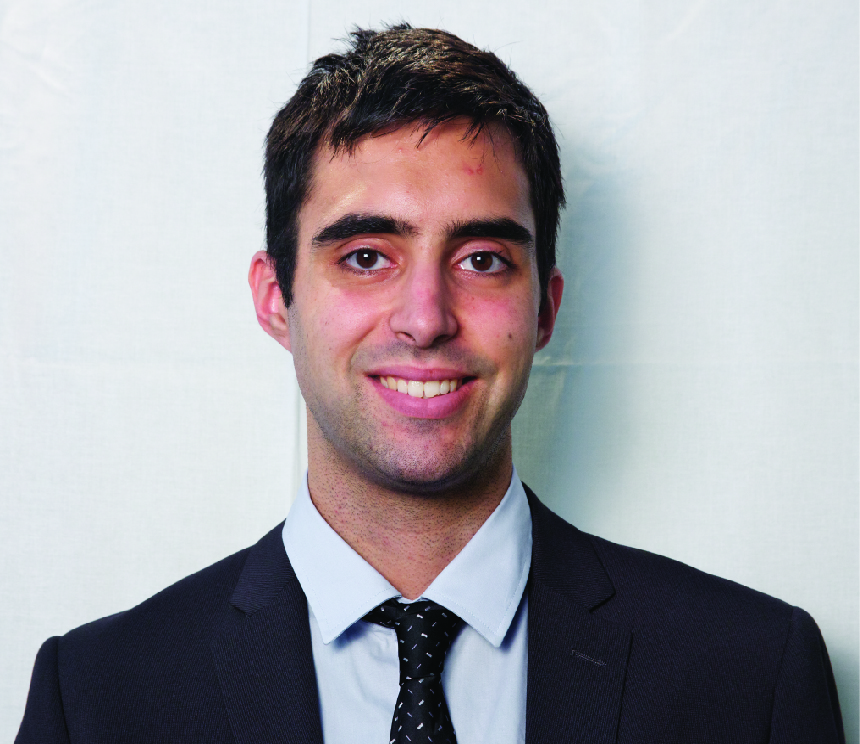
\includegraphics[trim= 320 130 460 210,clip,width=0.2\linewidth]{Foto_Smart.jpg}  %trimming relative to image size!
    %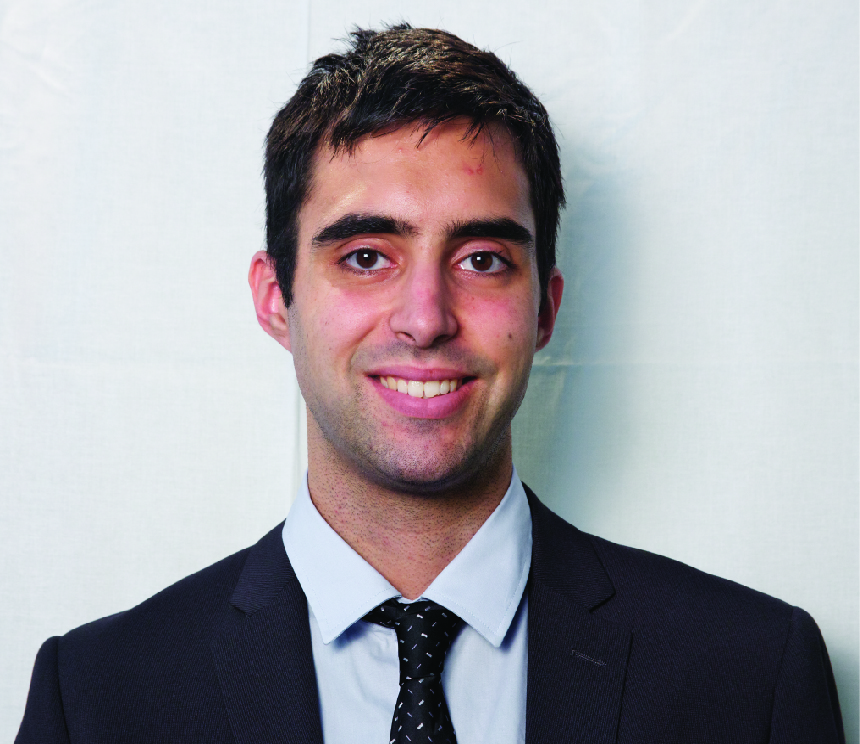
\includegraphics[width=0.2\linewidth]{Foto_Smart.jpg}
%\end{flushright}
%\end{figure}

%---------------------------------------------------------------------------------------
%  QR CODE (optional)
%----------------------------------------------------------------------------------------
%\vspace{-136pt}
%\hspace{0.75\linewidth}
%
\includegraphics[width=103pt]{qrcode}
%\normalsize
%\vspace{88pt}

%---------------------------------------------------------------------------------------
%  META SECTION
%----------------------------------------------------------------------------------------

%\vspace{-114pt}

%\metasection{Status:}{M.Sc. Digital Media, IT Consultant at We4IT Bremen}
%\metasection{Fields:}{Project Management, Software Development, Scrum, Usability}
%\metasection{Prefers:}{JS, Java, XPages, Flex / AIR, Processing, Git, Eclipse}
%\metasection{Activities:}{Global Game Jam, Sound Engineering, Blender, Martial Arts}

%\vspace{6pt}

%---------------------------------------------------------------------------------------
%  SUMMARAY (optional)
%----------------------------------------------------------------------------------------

%\cvsection{Summary}\\
%Digital media graduate with four years project experience in the field of technology based assessment. Specialized in development of test-scenario engines and innovative, rich media item formats. Master studies focused on teams from different disciplines and cultural backgrounds on solutions for complex problems.  Prior knowledge has been collected in he field of usability / accessibility during bachelor studies.\\

%============================================================================%
%
%  CV SECTIONS AND EVENTS (MAIN CONTENT)
%
%============================================================================%

%---------------------------------------------------------------------------------------
%  EDUCATION SECTION
%--------------------------------------------------------------------------------------
\cvsection{Formazione}

\cvevent{2017 - 2020}%
        {Dottorato in matematica applicata}%
        {\'Ecole des Ponts ParisTech, INRIA, EDF R\&D}%
        {\href{https://tel.archives-ouvertes.fr/tel-03080530}{Schemi \emph{Compatible Discrete Operator} per le equazioni non-stazionarie di Navier--Stoker per un fluido incompressibile}}%
        {Tutor: Ern Alexandre (ENPC, INRIA) e Bonelle J\'er\^ome (EDF R\&D)}%

\cvevent{2015 - 2017}%
        {Laurea Magistrale}%
        {Politecnico di Milano}%
        {\href{https://www.politesi.polimi.it/handle/10589/133692}{Ingegneria Matematica, specializzazione:} Scienze Computazionali per l'Ingegneria}%
        {Voto di Laurea: 110 e Lode/110}

%\textcolor{softcol}{\hrule}

%
\cvevent{2013 - 2017}%
        {Ciclo  dell'Ingegner \textit{Polytechnicien}}%
        {École polytechnique}%
        {Palaiseau, Francia. Equivalente a BSc e MSc}%
        {Specializzazione: Matematica Applicata -- EDP}

%\textcolor{softcol}{\hrule}

%
\cvevent{2010 - 2015}%
        {Laurea Triennale}%
        {Politecnico di Milano}%
        {Ingegneria Matematica. Voto di Laurea: 110 e Lode/110}%
        {Premio "Miglior Matricola" (2010) dopo i risultati del test d'ingresso e degli esami del primo semestre}

%---------------------------------------------------------------------------------------
%  EXPERIENCE
%----------------------------------------------------------------------------------------
\cvsection{Esperienze professionali}

%
\cvevent{09/'16-02/'17}%
        {Stage di Ricerca, 6 mesi}%
        {\href{https://www.politesi.polimi.it/handle/10589/133692}{EDF R\&D, Chatou}{Sviluppo e analisi numerica di un metodo HHO per i problemi di diffusione anisotropa}}%
        {Integrazione nel software industriale \cs{} (\texttt{C}); parallelizzazione con OpenMP}

%\textcolor{softcol}{\hrule}

%
\cvevent{03-08/2015}%
        {Stage di Ricerca, 5 mesi}%
        {US ESI R\&D, San Diego}%
        {Primi passi verso lo sviluppo di un nuovo sistema per un calcolo rapido della risposta vibro-acustica di un sistema}{Convalida con simulazioni}

%\textcolor{softcol}{\hrule}

%
\cvevent{08/2014}%
        {Stage Estivo}%
        {VTB Bank, Inkutsk}%
        {Foreign Exchange Control Group}%
        {Aiuto nella preparazione e convalida finale di contratti internazionali, gestione d'archivio}

\vspace{12pt}
\begin{minipage}{.48\linewidth}
\begin{flushleft}
\cvsubsection{Competenze informatiche}
\vspace{6pt}
\begin{tabular*}{1\linewidth}{l l}
&     \larrow{bgcol} \textbf{Buone}: \texttt{C}/\texttt{C++}, OpenMP, MPI, \href{https://github.com/RiMillo/LaTeX_tips}{\LaTeX}, sistemi Unix,\\[3pt]
  &       MATLAB/Scilab, Git/SVN, \href{https://www.code-saturne.org/cms/}{\cs{}}, Office\\[3pt]
&     \larrow{bgcol} \textbf{Basiche}: Python, shell script, FreeFem\texttt{++}, Fortran,\\[3pt]
&       Salome, Java, R
  \end{tabular*}
\end{flushleft}
\end{minipage}
\hfill
\begin{minipage}{.48\linewidth}
\begin{flushright}
\cvsubsection{Lingue}
\vspace{6pt}
\begin{tabular*}{1\linewidth}{l l l}
&     \larrow{bgcol} \textbf{Italiano}: &Madrelingua\\[3pt]
&     \larrow{bgcol} \textbf{Inglese}:  &Fluente, certificazione FCE, B2\\[3pt]
&     \larrow{bgcol} \textbf{Francese}: &Fluente, certificazione TCF, C1\\[3pt]
&     \larrow{bgcol} \textbf{Russo}:    &Livello base\\[3pt]
  \end{tabular*}
\end{flushright}
\end{minipage}

\bigskip

\begin{minipage}{.48\linewidth}
\begin{flushleft}
\cvsubsection{Attività extracurriculari}
\vspace{6pt}
\begin{tabular*}{1\textwidth}{l l}
&     \larrow{bgcol} Gestione di un dormitorio di studenti ('15) \\[3pt]
&     \larrow{bgcol} Tesoriere dell'\href{https://www.aim-mate.it/it/}{AIM} ('16)\\[3pt]
&     \larrow{bgcol} Rappresentante dei dottorandi EDF-MFEE ('18-'20) \\[3pt]
&     \larrow{bgcol} Running (maratona di Parigi '19)\\[3pt]
  \end{tabular*}
\end{flushleft}
\end{minipage}
\hfill
\begin{minipage}{.48\linewidth}
\begin{flushright}
\cvsubsection{Volontariato e altri Interessi}
\vspace{6pt}
\begin{tabular*}{1\linewidth}{l l}
&     \larrow{bgcol} Campi estivi (Kenya '10, '11; Ruanda '17)\\[3pt]
&     \larrow{bgcol} Membro di Smileland, che sostiene \\[3pt]
&       un villaggio di orfani in Congo\\[3pt]
&     \larrow{bgcol} Insegnamento di italiano per i profughi ('15-'16)\\[3pt]
  \end{tabular*}
\end{flushright}
\end{minipage}




%-------------------------------------------------------------------------------------------------
%  ARTIFICIAL FOOTER (fancy footer cannot exceed linewidth)
%--------------------------------------------------------------------------------------------------

\null
\vspace*{\fill}
%\hspace{-0.25\linewidth}\colorbox{bgcol}{\makebox[1.5\linewidth][c]{\mystrut \small \textcolor{white}{www.jankuester.com} $\cdot$ \textcolor{white}{github.com/jankapunkt}}}




%============================================================================%
%
%
%
%  DOCUMENT END
%
%
%
%============================================================================%
\end{document}
